\documentclass[class=minimal,border=0pt]{standalone}
\usepackage{tikz}
\usepackage{amsmath}

\usetikzlibrary{%
  arrows,
  calc
}
\usetikzlibrary{decorations.markings}
\usetikzlibrary{shapes.misc}

\begin{document}
  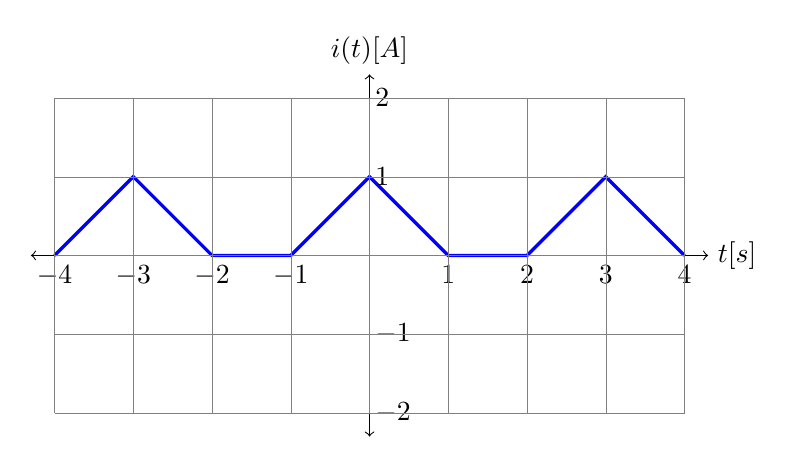
\begin{tikzpicture}[yscale=1, xscale=1]
    \draw[<->] (-4.3,0) -- (4.3,0) node[right] {$t[s]$};
    \draw[<->] (0,-2.3) -- (0,2.3) node[above] {$i(t)[A]$};

    \draw[line width = 1.2pt, blue] (-4,0) -- (-3,1) -- (-2,0)
    --  (-1,0) -- (0,1) -- (1,0)--(2,0)--(3,1)--(4,0);    
    
    
    \draw (-1,0) node[below] {$-1$};
    \draw (1,0) node[below] {$1$};
    \draw (-2,0) node[below] {$-2$};
    \draw (2,0) node[below] {$2$};
    \draw (3,0) node[below] {$3$};
    \draw (-3,0) node[below] {$-3$};
    \draw (4,0) node[below] {$4$};
    \draw (-4,0) node[below] {$-4$};
    

    \draw (-0.05,2) node[right] {$2$};
    \draw (-0.05,1) node[right] {$1$};
    \draw (-0.05,-1) node[right] {$-1$};
    \draw (-0.05,-2) node[right] {$-2$};
    

    \draw[step=1cm,color=gray, ultra thin] (-4,-2) grid (4,2);

  \end{tikzpicture}

\end{document}